\section{Task 1: Mapping natural language to web elements}
\label{sec:webrep}

\begin{figure}[t]
\centering
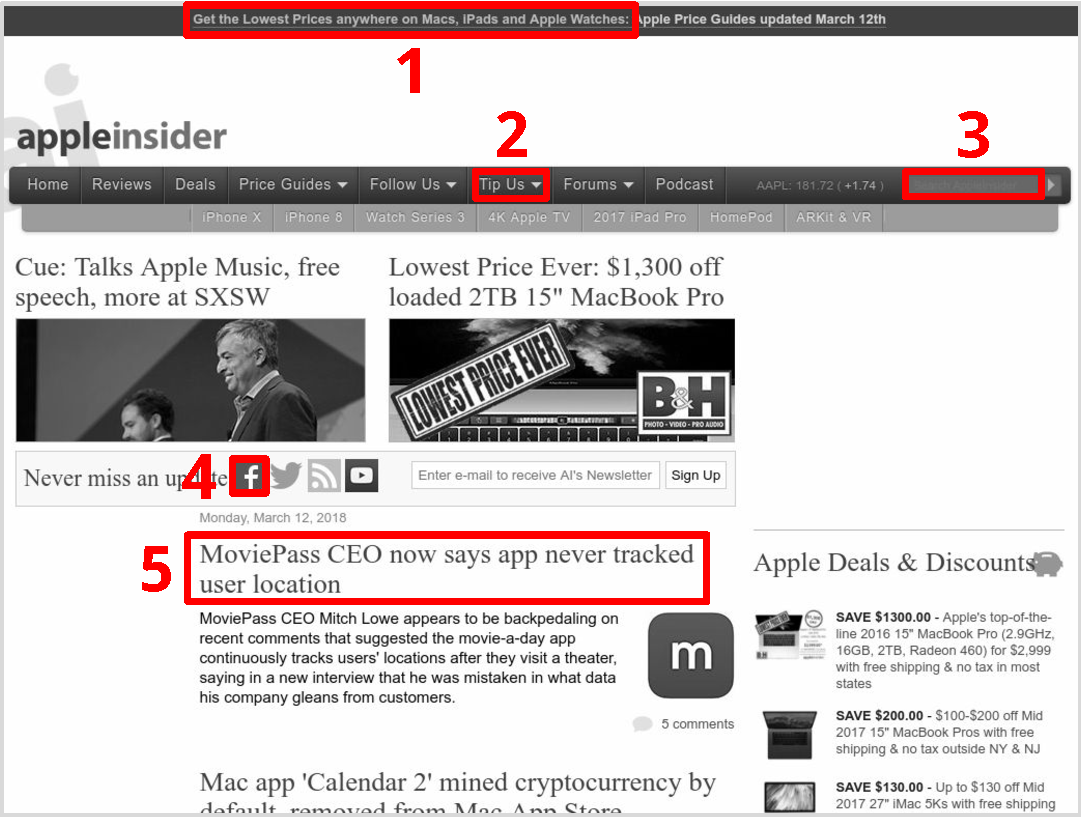
\includegraphics[width=0.7\textwidth]{figures/webrep/emnlp18-main-figure-alt.pdf}\\[.5em]
\begin{tabular}{@{}r@{\;}lr@{\;}l@{}}
1: & click on apple deals &
2: & send them a tip \\
3: & enter iphone 7 into search &
4: & follow on facebook \\
5: & open most recent news update \\
\end{tabular}
\caption{Examples of natural language commands on the web page \T{appleinsider.com}.}
\label{fig:webrep-running-ex}
\end{figure}

The first task we consider is the task of mapping
natural language commands to HTML elements on the web page
(e.g., links, buttons, and form inputs),
as illustrated in Figure~\ref{fig:webrep-running-ex}.
While some commands explicitly refer to the \emph{text content}
of the element, many others require considering other properties
of the element, as well as how the element relates to its context.

Our original motivation for the task was to make
web automation tools more robust.
Most automation tools rely on element selectors
such as CSS or XPath,
which rely on specific properties of the elements
(e.g., \T{id} or \T{class} attributes,
or the text content of the element).
While such explicit selectors can be easily interpreted
and edited by humans,
they struggle to generalize to other similar websites
or even different version of the same website
\cite{hammoudi2016why}.
We argue that natural language is a better
representation for the semantics of the web element,
and thus is more robust to cosmetic changes
(e.g., when the button text changes from \nl{Search} to \nl{Go!},
or when the \nl{Date} field moves to a different location on the page).
Apart from automation,
identifying elements via natural language
also has potential applications in
voice-enabled personal assistants
and assistive technology for the visually impaired
\cite{zajicek1998blind,ashok2014wizard}.

We first formalize the task and analyze the dataset
we collected for the task.
Afterward, we present three models for tackling the task:
\begin{itemize}
\item
The baseline \emph{retrieval-based model}
selects elements based on how well their text contents
and attributes match the input command.
\item
To allow inexact text matching,
the \emph{alignment-based model}
uses distributional similarity to compare the text tokens
in the element and the command.
\item
To incorporate other properties of the element,
the \emph{embedding-based model} encodes the attributes,
styles, and visual features of the element
and compares the result with the command.
\end{itemize}
Finally, we end the section with experimental results
and error analysis.

\paragraph{Reference.}
The results described in this section have been published as
\citet{pasupat2018elements}.
Reproducible experiments are hosted on the
CodaLab platform at
\begin{center}
\small
\url{https://worksheets.codalab.org/worksheets/0x0097f249cd944284a81af331093c3579}.
\end{center}

\subsection{Setup}

\paragraph{Task.}
Given a web page $w$ with HTML elements
$e_1, \dots, e_k$
and a natural language command $x$,
the system should
identify the element $e \in \set{e_1, \dots, e_k}$
described by $x$.
The training data contains $(w, x, e)$ tuples.

As illustrated in Figure~\ref{fig:webrep-running-ex},
the commands can reference the elements in various ways.
We collected a dataset containing commands with
interesting phenomena
using crowd sourcing, as described below.

\paragraph{Dataset.}
For our experiments,
we collected a dataset of 51,663 commands
on 1,835 web pages.
The data is collected as follows:
\begin{enumerate}
\item
We archived the home pages of top 10,000 websites
from Majestic Million.\footnote{\url{https://majestic.com/reports/majestic-million}}
We rendered each web page in Google Chrome
and waited for the dynamic content to load.
The post-rendering HTML and CSS files
were then recorded.
For each HTML element,
we also recorded all its HTML attributes
(e.g., \T{id} = \T{"new\_logo"}),
CSS properties
(e.g., \T{background-color} = \T{black}), bounding box size,
and the absolute position on the page.

\item
We manually filtered for around 2,000 web pages
that (a) are in English,
(b) are rendered properly,
and (c) do not contain inappropriate content.

\item
On each web page,
we asked crowd workers on Amazon Mechanical Turk
to describe a few actions to be performed on the page
(e.g., click on a link or fill in a form field).
Each action must involve exactly one HTML element
from the filtered list of interactive elements,\footnote{
We used the element filter from the Vimium project
(\url{https://vimium.github.io/})
with some slight simplification.}
which include visible links, form inputs, and buttons.
To encourage diversity,
we gave a bonus when the written description does not contain
the exact words from the text of the selected HTML element.

\end{enumerate}

The dataset is split into 70\% training,
10\% development, and 20\% test examples.
To test the model's ability to generalize to new environments,
we ensured that the web pages in the three sets do not overlap.
The web pages contain an average of 1,051 elements,
122 of which are considered interactive elements,
while the commands are 4.1 tokens long on average.

\begin{table}[t]
\centering
% \begin{tabular}{|l|p{4.8cm}|p{5cm}|r|}\hline
% \textbf{Phenomenon} & \textbf{Description} & \textbf{Example} & \textbf{Count} \\ \hline
% substring match &
% The command contains only a substring of the element's text (after stemming). &
% \nl{view internships with energy.gov} $\to$ ``Careers \& Internship link &
% 7.0 \% \\ \hline
% paraphrase &
% The command paraphrases the element's text. &
% \nl{click sign in} $\to$ ``Login'' link &
% 15.5 \% \\ \hline
% goal description &
% The command describes an action or asks a question. &
% \nl{change language} $\to$ a clickable box with text ``English'' &
% 18.0 \% \\ \hline
% summarization &
% The command summarizes the text in the element. &
% \nl{go to the article about the bengals trade}
% $\to$ the article title link &
% 1.5 \% \\ \hline
% element description &
% The command describes a property of the element. &
% \nl{click blue button} &
% 2.0 \% \\ \hline
% relational reasoning &
% The command requires reasoning with another element or its surrounding context. &
% \nl{show cookies info}
% $\to$ ``More Info'' in the cookies warning bar, not in the news section &
% 2.5 \% \\ \hline
%   ordinal reasoning &
% The command uses an ordinal. &
% \nl{click on the first article} &
% 3.5 \% \\ \hline
% spatial reasoning &
% The command describes the element's position. &
% \nl{click the three slashes at the top left of the page} &
% 2.0 \% \\ \hline
% image target &
% The target is an image (no text). &
% \nl{select the favorites button} &
% 11.5 \% \\ \hline
% form input target &
% The target is an input (text box, check box, drop-down list, etc.). &
% \nl{in the search bar, type testing} &
% 6.5 \% \\ \hline
% \end{tabular}

\begin{tabular}{llr}\toprule
\textbf{Phenomenon} & \textbf{Description and example} & \textbf{Count} \\ \midrule
substring match
& The command has only a substring of the element's text {\small(after stemming)}.
& 7.0 \% \\
& \nl{view internships with energy.gov}
$\to$ \nl{Careers \& Internship} link \\
%
paraphrase
& The command paraphrases the element's text.
& 15.5 \% \\
& \nl{click sign in}
$\to$ \nl{Login} link \\
%
goal description
& The command describes an action or asks a question.
& 18.0 \% \\
& \nl{change language}
$\to$ a clickable box with text \nl{English} \\
%
summarization
& The command summarizes the text in the element.
& 1.5 \% \\
& \nl{go to the article about the bengals trade}
$\to$ the article title link \\
%
element description
& The command describes a property of the element.
& 2.0 \% \\
& \nl{click blue button} \\
%
relational reasoning
& The command requires reasoning with its context. %another element or its surrounding context. &
& 2.5 \% \\
& \nl{show cookies info}
$\to$ \nl{More Info} in the cookies warning bar, \\
& \hspace*{9.8em} not the news section \\
%
ordinal reasoning
& The command uses an ordinal.
& 3.5 \% \\
& \nl{click on the first article} \\
%
spatial reasoning 
& The command describes the element's position.
& 2.0 \% \\
& \nl{click the three slashes at the top left of the page} \\
%
image target
& The target is an image (no text).
& 11.5 \% \\
& \nl{select the favorites button} \\
%
form input target
& The target is an input (e.g., text box, check box, drop-down list)
& 6.5 \% \\
& \nl{in the search bar, type testing} \\ \bottomrule
\end{tabular}
\caption[
Phenomena present in the dataset of mapping commands to web elements]{
Phenomena present in the commands in the dataset.
Each example can have multiple phenomena.}
\label{tab:webrep-phenomena}
\end{table}

\paragraph{Data analysis.}
We analyzed 200 examples from the training data
and broke down the type of reasoning present in these commands.
The statistics in Table~\ref{tab:webrep-phenomena} shows that
apart from using the exact text of the element,
commands can refer to the elements in a variety of ways.

Even when the command directly uses the text
of the element, many other elements on the same web page
also have word overlap with the command,
making the task not trivial.
On average, commands have word overlap (excluding stop words)
with 5.9 leaf elements on the page.

%%%%%%%%%%

\subsection{Representation of a web page}
We use the Document Object Model (DOM)
to represent the given web page $w$
as a tree of objects.
Unlike the HTML DOM standard which includes multiple types of nodes
(e.g., text nodes and comment nodes),
we use a simplified representation
where all tree node are element nodes.
As shown in Figure~\ref{fig:webrep-element-props},
each element node $e$ has various properties:

\begin{itemize}
\item \emph{Text content.}
The string inside the element.
(Concretely, we concatenate the text nodes from the original DOM tree,
using spaces as separators, to get the text content.)

\item \emph{Tags and attributes.}
Attributes such as \T{id} and \T{class} sometimes inform us
what the element's function is
(e.g., a Facebook social link usually has the substring \T{facebook}
in some of its attribute values).
However, some web pages use automatically-generated values for attributes
(e.g., \verb|id="u_ps_0_0_d"|).
To excel in this task, the system should try to learn the semantics
of meaningful attributes and ignore the spurious correlations
from automatic attribute values.

\item \emph{Visual features.}
After rendering the web page on a web browser,
we record the position, size, and visibility of the element,
as well as other styles
specified by Cascading Style Sheets (CSS).

\item \emph{Relations to other elements.}
In the DOM tree,
each element has at most one parent element
and zero or more child elements.
However, due to styling,
the structural relations in the DOM tree
does not necessarily reflect the visual relation
between elements.
Effectively taking visual relations into account is a challenging problem,
which we will defer as potential future work.
\end{itemize}

In the next three sections,
we describe our methods that take the properties
of HTML elements $e$ on the web page and determine the element
closest to the input command $x$.

\begin{figure}
\centering

\includegraphics[scale=0.5]{figures/webrep/features.png}
\verb|<a class="dd-head" id="tip-link" href="submit_story/">Tip Us</a>|
\\[1em]
\begin{tabular}{rl}
\multicolumn{2}{c}{\textbf{Text content}} \\
\multicolumn{2}{c}{tip us} \\
\multicolumn{2}{c}{\textbf{String attributes}} \\
class: & dd-head \\
id: & tip-link \\
href: & submit\_story/ \\
\multicolumn{2}{c}{\textbf{Visual features}} \\
location: & (0.53, 0.08) \\
visible: & true\hphantom{owowhatsthis} \\
background-color: & black \\
\end{tabular}
\caption{Example properties of an HTML element.}
\label{fig:webrep-element-props}
\end{figure}

\subsection{Retrieval-based model}
Many commands $x$ refer to the elements $e$
by their text content.
As a baseline, we consider a simple retrieval-based model
that selects the element based on the td-idf score.
In this setup,
each element on the web page
is treated as a ``document''
to be retrieved by the command.

\paragraph{Term frequency (tf).}
We represent each element as a bag-of-tokens computed by
(1) tokenizing and stemming its \emph{text content},
and (2) tokenizing \emph{attributes}
(\T{id}, \T{class}, \T{placeholder},
\T{label}, \T{tooltip},
\T{aria-text}, \T{name},
\T{src}, and \T{href})
at punctuation marks and camel-case boundaries
(e.g., \T{"header-user-dropdown"} becomes
three tokens: \T{header}, \T{user}, and \T{dropdown}).

The tokens from attributes are surprisingly descriptive,
especially when the text content is empty.
For instance, a Facebook icon image
is likely to have the token \T{facebook}
in either the \T{class} or \T{href} attribute.
However, since the text content is generally
more reliable than the attributes,
we down-weight the frequencies
of the tokens from attributes
by a factor of $\alpha = 3$ (tuned on the development set).

\paragraph{Inverse document frequency (idf).}
Each element is treated as a ``document'',
and the document frequencies (df) are computed
over all elements in the training dataset.
The inverse document frequency of a token $t$
is $\mathrm{idf}(t) = 1 + \ln\frac{N}{1 + n_t}$,
where $N$ is the total number of elements across all web pages,
and $n_t$ is the number of elements with token $t$
in its text content or textual attributes.

\paragraph{Ranking.}
From the given web page,
we select the element
with the highest tf-idf score.
If multiple elements share the highest score,
we heuristically pick the one that appears the earliest
in the pre-order traversal of the DOM tree.

\subsection{Alignment-based model}

% One downside of the embedding-based model
% is that the tokens from $c$ and $e$
% do not directly interact in the scoring function.
The retrieval-based model depends on exact token matches
to retrieve the correct element.
However, as seen in Table~\ref{tab:webrep-phenomena},
the command $x$ can relate to the text content of the element $e$
in various ways.
To incorporate synonyms
(e.g., \nl{click \textbf{start}} $\to$ \nl{\textbf{Begin}} button),
functional references
(e.g., \nl{find who \textbf{created} the site} $\to$
\nl{\textbf{Credits}} link),
and other types of token-token relations,
we consider using continuous token representations
to compute the token alignment between the command
and the text content of the element.

\paragraph{Model.}
Let $s(x, e)$ be a scoring function
that measures how well the command $x$
matches the text content and attributes of element $e$.
Given a command $x$,
we can define a conditional distribution over
the elements $e_1,\dots,e_k$ on the web page as
\begin{equation}
p(e_i \mid x) \propto \exp\crab{s(x, e_i)}.
\end{equation}
We can then train the parameter of the scoring function
to maximize the log-likelihood of the correct element
in the training data.
At test time, we simply predict the element
$e \in \set{e_1,\dots,e_k}$ with the highest score
$s(x, e)$.

\paragraph{Computing alignment in the scoring function.}
%To incorporate token-token interaction,
We want the scoring function $s(x,e)$
to measure how well the tokens in $x$ align with the tokens in $e$.
Previous works
on comparing two sequences of text
use either unidirectional
or bidirectional attention mechanism
to model token alignments
\cite{seo2016bidaf,yin2016abcnn,xiong2017dynamic,yu2018qanet}.
In this work,
we opt for a simpler method based
on a single alignment matrix
similar to \cite{hu2014convolutional}
as described below.

Let $t(e)$ be the concatenation of tokens
from text content and attributes of $e$.
(We trimmed $t(e)$ to the first 10 tokens to save memory.)
We then construct a matrix $A(x,e)$
where each entry $A_{ij}(x, e)$ is the dot product
between the embeddings of the $i$th token of $x$
and the $j$th token of $t(e)$.
The token embeddings are initialized with GloVe vectors
\cite{pennington2014glove}.

The matrix $A(x,e)$ is then passed through a convolution network
to get a fixed-sized vector.
(The convolution network contains two layers of size $3 \times 3$
followed by a max-pooling layer of size $2 \times 2$.)
The result is concatenated with
the embedding of the HTML tag of $e$,
and then passed through a feedforward network
to get the final score $s(x, e)$.

% For training,
% we simply replace the scoring function in
% Equation~\ref{eqn:webrep-prob}
% with the alignment-based scoring above,
% and then train on the same objective.

\subsection{Embedding-based model}

The two previous models only consider the text content
and attributes of the element $e$.
To incorporate other information such as the location,
geometry, and styles of the element,
we propose the embedding-based model,
which embeds the different properties of the element
and compare the result with the embedding of the command.
% A common method for relating two pieces of texts
% is to embed them separately and then compute a score
% based on the two embeddings
% \cite{kiros2015skip,tai2015improved}
% \todo{Change the motivation}
Concretely,
for a command $x$ and elements $e_1, \dots, e_k$,
we define the following conditional distribution
over the elements:
\begin{equation}
p(e_i \mid x) \propto \exp\crab{s(f(x), g(e_i))},
\label{eqn:webrep-prob}
\end{equation}
where $s$ is a scoring function,
$f(x)$ is the embedding of $x$,
and $g(e_i)$ is the embedding of $e_i$.
Like the alignment-based model,
the embedding-based model is trained to maximize the log-likelihood
of the correct element in the training data.

\paragraph{Command embedding.}
We compute $f(x)$ by averaging the word embeddings
of the tokens in $x$.
The token embeddings are initialized with GloVe vectors
\cite{pennington2014glove}.
We also experimented with using recurrent neural network
but found no improvement.

\paragraph{Element embedding.}
To compute $g(e)$, we embed the properties of $e$,
concatenate the results, and then apply a feedforward
network to obtain a vector of the same size as $f(x)$.
The properties include:

\begin{itemize}
\item \emph{Text content.}
We apply the command embedder $f$ on the text content of $e$.
(The token embeddings are shared.)
As the text of most elements of interest
(links, buttons, and inputs) are short,
we limit the text to the first 10 tokens to save memory.

\item \emph{Text attributes.}
We consider the following attributes
which usually contain natural language:
\T{aria}, \T{title}, \T{tooltip},
\T{placeholder}, \T{label}, and \T{name}.
We concatenate the values and then apply the
command embedder $f$ on the resulting string.

\item \emph{Tag and symbolic attributes.}
The HTML tag, \T{id}, and \T{class}
are usually not in natural language
but are nevertheless informative.
We tokenize these strings at punctuation marks
and camel-case boundaries.
We then embed the tokens with separate embedding lookup tables
and then average the results.

\item \emph{Visual features.}
We construct a vector consisting of the coordinates of
the element's center (as fractions of the page width and height)
and visibility (as a boolean).

\end{itemize}

\paragraph{Scoring function.}
To compute the score $s(f(x), g(e_i))$,
we first normalize $f(x)$ and $g(e_i)$ into
unit-norm vectors $\hat f(x)$ and $\hat g(e_i)$.
We then apply a feedforward network on
the concatenation of $\hat f(x)$, $\hat g(e_i)$,
and $\hat f(x) \circ \hat g(e_i)$
(where $\circ$ denotes element-wise product).



\subsection{Experiments}
We evaluate the three approaches above on \emph{accuracy}:
the fraction of examples that the model selects
the correct element among all \emph{visible} elements
on the web page.
For training the neural models,
we use Adam \cite{kingma2014adam} with the initial
learning rate of $10^{-3}$ and early stopping.
%based on the development set.

The result in Table~\ref{tab:webrep-results}
shows that both neural models significantly
outperform the retrieval-based model.
The embedding-based model,
which also incorporates non-text properties of the elements,
outperforms the alignment-based model.
However, later in our error analysis,
we will show that
the alignment-based model is better at certain types
of commands than the encoding-based one.

\begin{table}[t]
\centering
\begin{tabular}{lr}\toprule
\textbf{Model} & \textbf{Accuracy (\%)} \\
\midrule
retrieval-based & 36.55 \\ %& 37.95 \\
\midrule
alignment-based & 50.74 \\ %& 50.94 \\
\hspace*{.5em} no texts & 15.94 \\ %& 15.63 \\
\hspace*{.5em} no attributes & 48.51 \\ %& 48.77 \\
%\hspace*{.5em} no spatial context  & 50.66 \\ %& 50.86 \\
\midrule
embedding-based & 56.05 \\ %& 56.35 \\ 
\hspace*{.5em} no texts & 23.62 \\ %& 23.84 \\
\hspace*{.5em} no attributes & 55.43 \\ %& 55.79 \\
%\hspace*{.5em} no spatial context & 58.87 \\ %& 59.13 \\
\bottomrule
\end{tabular}
\caption{Accuracy of the models and their ablations.
%\todo{Remove spatial context}
}
\label{tab:webrep-results}
\end{table}

\paragraph{Ablation.}
We perform an ablation study where the neural models
do not observe the text contents or the attributes.
Unsurprisingly, the results in Table~\ref{tab:webrep-results}
shows that text contents is the most crucial signal.
However, attributes also play an important role
in both embedding-based and alignment-based models.

\paragraph{Error analysis.}
To get a better picture of how the models handle
different phenomena,
we analyze the predictions of the embedding-based
and alignment-based models on 100 development examples
where at least one model made an error.
Table~\ref{tab:webrep-errors} summarizes
the error types, which are described in detail below:

\begin{table}[t]
\centering
\begin{tabular}{lrr}\toprule
\textbf{Error Type} & \textbf{Align} & \textbf{Embed} \\
\midrule
Fail to match strings & 11.6\% & 26.8\% \\
Incorrectly match strings & 14.2\% & 3.8\% \\
Fail to understand paraphrases & 7.9\% & 8.9\% \\
Fail to understand descriptions & 17.4\% & 12.1\% \\
Fail to perform reasoning & 13.7\% & 15.9\% \\
Select a less prominent element & 24.8\% & 19.8\% \\
Noisy annotation & 10.5\% & 12.7\% \\
\bottomrule
\end{tabular}
\caption[
Error breakdowns of the embedding and alignment models
on 100 examples.
]{
Error breakdowns of the embedding and alignment models
on 100 examples.
The embedding model handles implicit descriptions well, while
the alignment model excels at string matching.}
\label{tab:webrep-errors}
\end{table}

\begin{itemize}
\item \emph{Fail to match strings.}
Many commands simply specify the text content of the element
(e.g., \nl{click customised garages}
$\to$ the link with text
``Customised Garages, Canopies \& Carports'').
The embedding-based model
occasionally fails to select the element with partially matching texts.
In contrast, the alignment-based model
explicitly models text matching,
and thus is better at this type of commands.

\item \emph{Incorrectly match strings.}
However,
due to its reliance on text matching,
the alignment-based model struggles when many elements
share substrings with the command
(e.g., \nl{shop for knitwear} matches
many elements contain the word ``shop''),
or when an element with a matching substring is not the correct target
(e.g., \nl{get the program} was incorrectly mapped to
the ``Microsoft developer program'' link,
while the correct answer is the ``Download'' link).

\item \emph{Fail to understand descriptions.}
As seen in Table~\ref{tab:webrep-phenomena},
many commands indirectly describe the elements using paraphrases,
goal descriptions, or properties of the elements.
The embedding-based model summarizes
various properties of the elements
in the embedding $g(e)$,
making it better at handling these commands
than the alignment-based model.
However, the embedding-based model still makes
a few errors on harder examples
(e.g., for the command
\nl{please close this notice for me},
the model fails to select the ``X'' button
with hidden text ``Hide``).

\item \emph{Fail to perform reasoning.}
The proposed models do not handle
relational, ordinal, or spatial reasoning.
The most frequent error mode is when the element is a text box,
and the command uses nearby label as the reference
(e.g., \nl{type 94305 in the zip code field}
should map to the text box near the label ``Zip Code'').
While a few text boxes have semantic annotations
which the model can use
(e.g., \T{name}, \T{tooltip},
or \T{aria} attributes),
many web pages do not provide such annotations.
To handle these cases, a model would have to identify the label
of the text box based on logical or visual contexts.

\item \emph{Other errors.}
Apart from annotation errors,
occasionally multiple elements on the web page
satisfy the given command
(e.g., \nl{log in}
can match any ``Sign In'' button on the web page).
In these cases, the annotation usually gives the most \emph{prominent} element
among the possible candidates.
To provide a natural interface for users,
the model should arguably learn to predict such prominent elements
instead of more obscure ones.
\end{itemize}